\documentclass[tikz, border=6pt]{standalone}
\usepackage[T1]{fontenc}
\usepackage{lmodern}
\usepackage{amsmath,amssymb,bm}
\usepackage[scaled=0.95]{helvet}
\usetikzlibrary{arrows.meta}
\definecolor{Blue}{HTML}{3A76D8}
\definecolor{Green}{HTML}{3BA55C}
\definecolor{Yellow}{HTML}{EAB531}
\definecolor{Orange}{HTML}{EE8133}
\definecolor{Purple}{HTML}{8459D1}
\definecolor{Gray}{HTML}{6B7280}
\definecolor{Ink}{HTML}{1F2937}
\definecolor{cFBFBFB}{HTML}{FBFBFB}
\definecolor{cFBFCFC}{HTML}{FBFCFC}
\definecolor{cEDEDEF}{HTML}{EDEDEF}
\definecolor{cEAEBEC}{HTML}{EAEBEC}
\definecolor{cFAFAFA}{HTML}{FAFAFA}
\definecolor{cFFFFFF}{HTML}{FFFFFF}
\definecolor{c4C545F}{HTML}{4C545F}
\definecolor{c1F2937}{HTML}{1F2937}
\definecolor{c353E4B}{HTML}{353E4B}
\definecolor{cE6E7E8}{HTML}{E6E7E8}
\definecolor{cF1F2F2}{HTML}{F1F2F2}
\definecolor{cE5E6E7}{HTML}{E5E6E7}
\definecolor{cFDFDFD}{HTML}{FDFDFD}
\definecolor{cEEEFF0}{HTML}{EEEFF0}
\definecolor{cF4F5F6}{HTML}{F4F5F6}
\definecolor{cE9EAEB}{HTML}{E9EAEB}
\definecolor{cE7E8EA}{HTML}{E7E8EA}
\definecolor{c4F5762}{HTML}{4F5762}
\definecolor{c333C49}{HTML}{333C49}
\definecolor{cF2F2F3}{HTML}{F2F2F3}
\definecolor{cF4F4F5}{HTML}{F4F4F5}
\definecolor{cF5F6F6}{HTML}{F5F6F6}
\definecolor{cECEDEE}{HTML}{ECEDEE}
\definecolor{cEDEEEF}{HTML}{EDEEEF}
\definecolor{c3F4753}{HTML}{3F4753}
\definecolor{cF9F9FA}{HTML}{F9F9FA}
\definecolor{c3A434F}{HTML}{3A434F}
\definecolor{cEFF0F1}{HTML}{EFF0F1}
\definecolor{cF8F8F9}{HTML}{F8F8F9}
\definecolor{cE6E8E9}{HTML}{E6E8E9}
\definecolor{c58606A}{HTML}{58606A}
\definecolor{cF3F3F4}{HTML}{F3F3F4}
\tikzset{
  block/.style={/utils/exec={\colorlet{pytikzarg}{#1}}, draw=pytikzarg!78!black, fill=pytikzarg!14, rounded corners=3pt, align=center, inner sep=5pt, minimum height=8mm, minimum width=20mm},
  block/.default=Blue,
}
\begin{document}
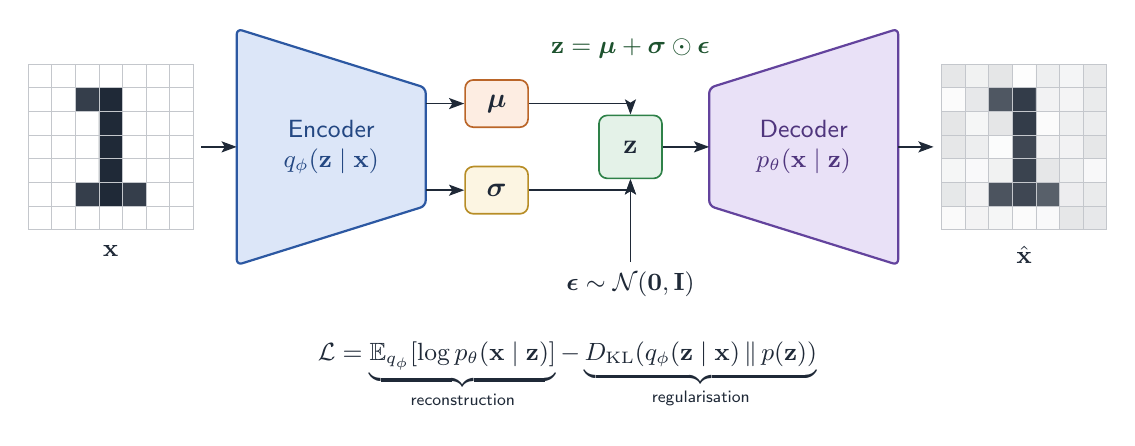
\begin{tikzpicture}[color=Ink, execute at begin picture={\sffamily}, line width=0.6pt, >={Stealth[length=5.5pt, width=4pt, inset=1.2pt]}, line join=round]
  % cell grid  7x7
  \fill[cFFFFFF] (-1.05,0.75) rectangle (-0.75,1.05) (-0.75,0.75) rectangle (-0.45,1.05) (-0.45,0.75) rectangle (-0.15,1.05) (-0.15,0.75) rectangle (0.15,1.05) (0.15,0.75) rectangle (0.45,1.05) (0.45,0.75) rectangle (0.75,1.05) (0.75,0.75) rectangle (1.05,1.05) (-1.05,0.45) rectangle (-0.75,0.75) (-0.75,0.45) rectangle (-0.45,0.75) (0.15,0.45) rectangle (0.45,0.75) (0.45,0.45) rectangle (0.75,0.75) (0.75,0.45) rectangle (1.05,0.75) (-1.05,0.15) rectangle (-0.75,0.45) (-0.75,0.15) rectangle (-0.45,0.45) (-0.45,0.15) rectangle (-0.15,0.45) (0.15,0.15) rectangle (0.45,0.45) (0.45,0.15) rectangle (0.75,0.45) (0.75,0.15) rectangle (1.05,0.45) (-1.05,-0.15) rectangle (-0.75,0.15) (-0.75,-0.15) rectangle (-0.45,0.15) (-0.45,-0.15) rectangle (-0.15,0.15) (0.15,-0.15) rectangle (0.45,0.15) (0.45,-0.15) rectangle (0.75,0.15) (0.75,-0.15) rectangle (1.05,0.15) (-1.05,-0.45) rectangle (-0.75,-0.15) (-0.75,-0.45) rectangle (-0.45,-0.15) (-0.45,-0.45) rectangle (-0.15,-0.15) (0.15,-0.45) rectangle (0.45,-0.15) (0.45,-0.45) rectangle (0.75,-0.15) (0.75,-0.45) rectangle (1.05,-0.15) (-1.05,-0.75) rectangle (-0.75,-0.45) (-0.75,-0.75) rectangle (-0.45,-0.45) (0.45,-0.75) rectangle (0.75,-0.45) (0.75,-0.75) rectangle (1.05,-0.45) (-1.05,-1.05) rectangle (-0.75,-0.75) (-0.75,-1.05) rectangle (-0.45,-0.75) (-0.45,-1.05) rectangle (-0.15,-0.75) (-0.15,-1.05) rectangle (0.15,-0.75) (0.15,-1.05) rectangle (0.45,-0.75) (0.45,-1.05) rectangle (0.75,-0.75) (0.75,-1.05) rectangle (1.05,-0.75);
  \fill[c353E4B] (-0.45,0.45) rectangle (-0.15,0.75) (-0.45,-0.75) rectangle (-0.15,-0.45) (0.15,-0.75) rectangle (0.45,-0.45);
  \fill[c1F2937] (-0.15,0.45) rectangle (0.15,0.75) (-0.15,0.15) rectangle (0.15,0.45) (-0.15,-0.15) rectangle (0.15,0.15) (-0.15,-0.45) rectangle (0.15,-0.15) (-0.15,-0.75) rectangle (0.15,-0.45);
  \draw[Gray!40, line width=0.3pt] (-1.05,-1.05) -- (1.05,-1.05) (-1.05,-0.75) -- (1.05,-0.75) (-1.05,-0.45) -- (1.05,-0.45) (-1.05,-0.15) -- (1.05,-0.15) (-1.05,0.15) -- (1.05,0.15) (-1.05,0.45) -- (1.05,0.45) (-1.05,0.75) -- (1.05,0.75) (-1.05,1.05) -- (1.05,1.05) (-1.05,-1.05) -- (-1.05,1.05) (-0.75,-1.05) -- (-0.75,1.05) (-0.45,-1.05) -- (-0.45,1.05) (-0.15,-1.05) -- (-0.15,1.05) (0.15,-1.05) -- (0.15,1.05) (0.45,-1.05) -- (0.45,1.05) (0.75,-1.05) -- (0.75,1.05) (1.05,-1.05) -- (1.05,1.05);
  \node[anchor=north, font=\small, align=center] at (0,-1.13) {$\mathbf{x}$};
  % cell grid  7x7
  \fill[cE6E7E8] (10.55,0.75) rectangle (10.85,1.05) (10.55,-0.15) rectangle (10.85,0.15) (12.35,-0.15) rectangle (12.65,0.15) (11.75,-0.45) rectangle (12.05,-0.15) (12.05,-1.05) rectangle (12.35,-0.75);
  \fill[cF1F2F2] (10.85,0.75) rectangle (11.15,1.05) (11.15,-0.45) rectangle (11.45,-0.15);
  \fill[cE5E6E7] (11.15,0.75) rectangle (11.45,1.05) (10.55,0.15) rectangle (10.85,0.45) (11.15,0.15) rectangle (11.45,0.45);
  \fill[cFDFDFD] (11.45,0.75) rectangle (11.75,1.05);
  \fill[cEEEFF0] (11.75,0.75) rectangle (12.05,1.05) (12.05,0.15) rectangle (12.35,0.45);
  \fill[cF4F5F6] (12.05,0.75) rectangle (12.35,1.05);
  \fill[cE9EAEB] (12.35,0.75) rectangle (12.65,1.05);
  \fill[cFBFBFB] (10.55,0.45) rectangle (10.85,0.75) (11.75,0.15) rectangle (12.05,0.45) (11.45,-1.05) rectangle (11.75,-0.75);
  \fill[cE7E8EA] (10.85,0.45) rectangle (11.15,0.75) (12.35,-1.05) rectangle (12.65,-0.75);
  \fill[c4F5762] (11.15,0.45) rectangle (11.45,0.75);
  \fill[c333C49] (11.45,0.45) rectangle (11.75,0.75) (11.45,0.15) rectangle (11.75,0.45);
  \fill[cF2F2F3] (11.75,0.45) rectangle (12.05,0.75) (11.75,-0.15) rectangle (12.05,0.15) (12.05,-0.15) rectangle (12.35,0.15) (10.85,-0.75) rectangle (11.15,-0.45);
  \fill[cF4F4F5] (12.05,0.45) rectangle (12.35,0.75);
  \fill[cEAEBEC] (12.35,0.45) rectangle (12.65,0.75) (12.35,-0.75) rectangle (12.65,-0.45);
  \fill[cF5F6F6] (10.85,0.15) rectangle (11.15,0.45) (10.55,-0.45) rectangle (10.85,-0.15) (11.15,-1.05) rectangle (11.45,-0.75);
  \fill[cECEDEE] (12.35,0.15) rectangle (12.65,0.45);
  \fill[cEDEEEF] (10.85,-0.15) rectangle (11.15,0.15);
  \fill[cFBFCFC] (11.15,-0.15) rectangle (11.45,0.15);
  \fill[c3F4753] (11.45,-0.15) rectangle (11.75,0.15) (11.45,-0.75) rectangle (11.75,-0.45);
  \fill[cF9F9FA] (10.85,-0.45) rectangle (11.15,-0.15) (11.75,-1.05) rectangle (12.05,-0.75);
  \fill[c3A434F] (11.45,-0.45) rectangle (11.75,-0.15);
  \fill[cEFF0F1] (12.05,-0.45) rectangle (12.35,-0.15);
  \fill[cF8F8F9] (12.35,-0.45) rectangle (12.65,-0.15);
  \fill[cE6E8E9] (10.55,-0.75) rectangle (10.85,-0.45);
  \fill[c4C545F] (11.15,-0.75) rectangle (11.45,-0.45);
  \fill[c58606A] (11.75,-0.75) rectangle (12.05,-0.45);
  \fill[cEDEDEF] (12.05,-0.75) rectangle (12.35,-0.45);
  \fill[cFAFAFA] (10.55,-1.05) rectangle (10.85,-0.75);
  \fill[cF3F3F4] (10.85,-1.05) rectangle (11.15,-0.75);
  \draw[Gray!40, line width=0.3pt] (10.55,-1.05) -- (12.65,-1.05) (10.55,-0.75) -- (12.65,-0.75) (10.55,-0.45) -- (12.65,-0.45) (10.55,-0.15) -- (12.65,-0.15) (10.55,0.15) -- (12.65,0.15) (10.55,0.45) -- (12.65,0.45) (10.55,0.75) -- (12.65,0.75) (10.55,1.05) -- (12.65,1.05) (10.55,-1.05) -- (10.55,1.05) (10.85,-1.05) -- (10.85,1.05) (11.15,-1.05) -- (11.15,1.05) (11.45,-1.05) -- (11.45,1.05) (11.75,-1.05) -- (11.75,1.05) (12.05,-1.05) -- (12.05,1.05) (12.35,-1.05) -- (12.35,1.05) (12.65,-1.05) -- (12.65,1.05);
  \node[anchor=north, font=\small, align=center] at (11.6,-1.13) {$\hat{\mathbf{x}}$};
  \draw[fill=Blue!18, draw=Blue!75!black, line width=0.8pt, rounded corners=2pt] (1.6,-1.5) --
      (4,-0.75) -- (4,0.75) -- (1.6,1.5) -- cycle;
  \node[align=center, font=\small, text=Blue!60!black] at (2.8,0) {Encoder\\$q_\phi(\mathbf{z}\mid\mathbf{x})$};
  \draw[fill=Purple!18, draw=Purple!75!black, line width=0.8pt, rounded corners=2pt] (7.6,-0.75) --
      (10,-1.5) -- (10,1.5) -- (7.6,0.75) -- cycle;
  \node[align=center, font=\small, text=Purple!60!black] at (8.8,0) {Decoder\\$p_\theta(\mathbf{x}\mid\mathbf{z})$};
  \node[block=Orange, minimum width=0.8cm, minimum height=0.6cm] (n1) at (4.9,0.55) {$\boldsymbol{\mu}$};
  \node[block=Yellow, minimum width=0.8cm, minimum height=0.6cm] (n2) at (4.9,-0.55) {$\boldsymbol{\sigma}$};
  \node[block=Green, minimum width=0.8cm, minimum height=0.8cm] (n3) at (6.6,0) {$\mathbf{z}$};
  \node[font=\small] (n4) at (6.6,-1.75) {$\boldsymbol{\epsilon}\sim\mathcal{N}(\mathbf{0}, \mathbf{I})$};
  \draw[->] (1.15,0) -- (1.6,0);
  \draw[->] (4,0.55) -- (n1.west);
  \draw[->] (4,-0.55) -- (n2.west);
  \draw[->] (n1.east) -| (n3);
  \draw[->] (n2.east) -| (n3);
  \draw[->] (n4) -- (n3.south);
  \draw[->] (n3.east) -- (7.6,0);
  \draw[->] (10,0) -- (10.45,0);
  \node[font=\small, text=Green!50!black] at (6.6,1.25) {$\mathbf{z} = \boldsymbol{\mu} + \boldsymbol{\sigma}\odot\boldsymbol{\epsilon}$};
  \node[font=\small] at (5.8,-2.9) {$\mathcal{L} = \underbrace{\mathbb{E}_{q_\phi}\!\left[\log p_\theta(\mathbf{x}\mid\mathbf{z})\right]}_{\text{reconstruction}} - \underbrace{D_{\mathrm{KL}}\!\left(q_\phi(\mathbf{z}\mid\mathbf{x})\,\|\,p(\mathbf{z})\right)}_{\text{regularisation}}$};
\end{tikzpicture}
\end{document}
